% 大学物理实验报告

\documentclass[UTF8]{ctexart}

\usepackage{amsmath}        %数学公式
\usepackage{cases}          %联立编号
\usepackage{cite}           %引用
% \usepackage{enumitem}       %编号

\usepackage{graphicx}       %插入图片
\usepackage{float}          %设置图片浮动位置
\usepackage{subfigure}      %插入多图时用子图显示

\usepackage{anyfontsize}    %解决一个奇怪的字体大小报错问题
\usepackage{fancyhdr}       %页眉、页脚、页码
\usepackage[a4paper, margin=1in]{geometry}    %纸张大小


\setlength{\headheight}{16pt}
\pagestyle{fancy}
\fancyhf{}


\title{霍尔效应及磁阻测量实验报告}
\author{\LaTeX\ by\ Jerry\ }
\date{\today}
\pagenumbering{arabic}

\begin{document}

\fancyhead[L]{Jerry}
\fancyhead[C]{霍尔效应及磁阻测量实验}
\fancyfoot[C]{\thepage}

\maketitle
\newpage
\tableofcontents
\newpage

\section{实验目的}

\begin{enumerate}
    \item 了解霍尔效应及其副效应的产生原理
    \item 掌握霍尔系数的测量方法,学习消除霍尔副效应的实验方法
    \item 研究半导体材料的电阻值随磁场的变化规律
\end{enumerate}

\section{实验原理}

\subsection{霍尔效应}

如图\ref{Hall_effect},通电流的导体置于磁场$B$中,磁场方向垂直于电流$I$方向,观察电压表$G$可以发现产生垂直于电流方向和磁场方向的电位差$U_H$,这就是霍尔效应。

\begin{center}
    \begin{figure}[H]
        \centering
        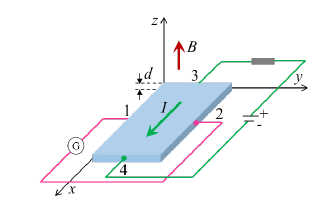
\includegraphics[width=0.3\textwidth]{img/Hall_effect.png}
        \caption{霍尔效应示意图}
        \label{Hall_effect}
    \end{figure}
\end{center}

如图\ref{Hall_voltage},可以发现载流子在磁场中受到洛仑兹力偏转,导致电子在$y$方向积累,产生电场,使电子受到洛仑兹力和电场力平衡,从而产生霍尔电压。

\begin{center}
    \begin{figure}[H]
        \centering
        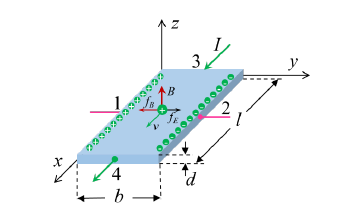
\includegraphics[width=0.3\textwidth]{img/Hall_voltage.png}
        \caption{霍尔电压示意图}
        \label{Hall_voltage}
    \end{figure}
\end{center}

通过推导可以得出:霍尔电压$U_H$与电流$I$、磁感应强度$B$、样品几何尺寸有关,其表达式为:$$U_H = K_H\frac{IB}{d}$$其中$K_H$为霍尔系数,$d$为样品厚度。

\subsection{霍尔效应的副效应}

\subsubsection{厄廷好森(Etinghausen)效应}

霍尔电压$U_H$与样品温度$T$有关,其表达式为:$U_H = U_{H0} + \alpha(T-T_0)$。
其中$U_{H0}$为$T_0$时的霍尔电压,$\alpha$为霍尔电压的温度系数。

\subsubsection{能斯脱(Nernst)效应}

由于连接点$3$、$4$处的接触电阻可能不同,使得电极$3$和$4$两点的温度不同,
引起载流子在$x$方向的运动产生热流,它在磁场作用下在$1$和$2$两点间产生电位差$U_N$。
$U_N$的符号只与磁场$B$的方向有关。

\subsubsection{里纪-勒杜克(Righi-Leduc)效应}

上述热流中的载流子的速度各不相同,在磁场作用下也会使$1$和$2$两点间出现温差电动势$U_R$。
则$U_R$的方向只与$B$的方向有关。

\subsubsection{不等位效应所引起的电位差$U_0$}

由于制作工艺上的困难,$1$、$2$两点不可能恰好处在同一条等位线上,因而只要样品中有电流通过,
$1$和$2$两点间就会出现电位差$U_0$。$U_0$的正负只与工作电流的方向有关。

\subsubsection{电压表附加电压$U_S$}

$U_S$是与电流方向和磁场方向无关的量

\subsection{副效应的消除方法}

通过改变工作电流$I$的方向和外加磁场$B$的方向的不同组合测量可以消除或减少$U_N$、$U_R$和$U_0$的影响。
$U_E$变化与$U_H$变化相同,但是$U_E$远小于$U_H$,可以忽略不计。通过减少通电流时间可以减少温度变化造成的干扰。

参考图\ref{Hall_voltage},让电流$I$沿$x$正方向(3$\to$4),磁场$B$沿$z$正方向,此时测得$1$、$2$间的电压为$U_{1}(+B,+I)$。
保持磁场方向不变,改变电流方向为$x$负方向(4$\to$3),此时测得$1$、$2$间的电压为$U_{2}(+B,-I)$。
再依次改变磁场方向为$z$负方向,$x$负方向,$z$正方向,$x$正方向,测得$U_{3}(-B,-I)$,$U_{4}(-B,+I)$。
则霍尔电压为:$$U_H = \frac{1}{4}|U_1-U_2+U_3-U_4|$$

\subsection{磁电阻效应}

电流方向和磁场方向互相垂直,载流子将受洛伦兹力的作用,发生偏转,在$AB$两端产生积聚电荷
并形成霍尔电场。如果霍尔电场作用和某一速度的载流子受到的洛伦兹力作用刚好抵消,
那么小于或大于该速度的载流子将发生偏转。因此沿外加电场方向运动的载流子数目将减少,
电阻增大,表现出横向磁电阻效应(这里的横向指的是电流方向和磁场方向互相垂直)。如果将
$A$、$B$端短接,则霍尔电场将不存在,所有电子将向$A$端偏转,也表现出横向磁电阻效应。

\section{实验仪器}

实验装置台号:12

\begin{center}
    \begin{figure}[H]
        \centering
        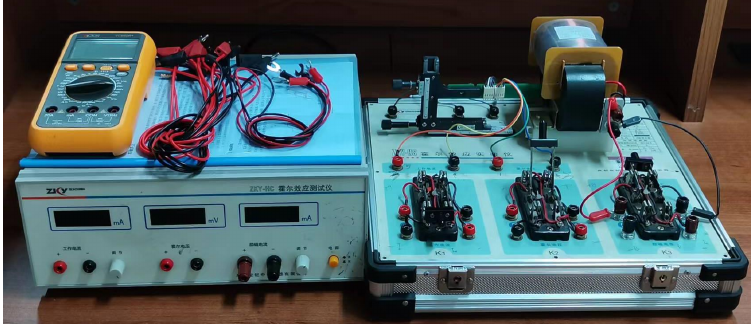
\includegraphics[width=0.6\textwidth]{img/Device.png}
        \caption{实验装置}
        \label{Device}
    \end{figure}
\end{center}

如图\ref{Device}所示,共使用了以下仪器:

\begin{itemize}
    \item ZKY-HC霍尔效应测试仪
    \begin{itemize}
        \item 霍尔元件电流 $I$ : 1.50\~{}10.00mA
        \item 霍尔电压电表量程 : 199.9mV
        \item 激磁电流 $I_M$ : 0\~{}1000mA
    \end{itemize}
    \item VICTOR数字万用表VC9806+
    \begin{itemize}
        \item 量程 : 1.999V
    \end{itemize}
    \item 霍尔效应实验仪-No.110845
    \begin{itemize}
        \item 霍尔元件参数:
        \begin{itemize}
            \item $K_H$(mV/mA.T) = 19
            \item $V_0$(mV) = 0
            \item $R_{in}$($\Omega$) = 87
            \item $R_{out}$($\Omega$) = 100.5
            \item 材料 = N型GaN
            \item 霍尔片尺寸 : $l$ = 300$\mu$m,$b$ = 100$\mu$m,$d$ = 3$\mu$m
        \end{itemize}
        \item 电磁铁参数:
        \begin{itemize}
            \item 横截面积(mm) = 40$\times$20.5
            \item 气隙(mm) = 8
            \item 周长(mm) = 内234,外348
            \item 匝数 = 1743
            \item 线径(mm) = 0.63
        \end{itemize}
    \end{itemize}
    \item 导线若干
\end{itemize}

\section{实验步骤}

\subsection{霍尔效应实验研究}

\subsubsection{测量霍尔片的有关参数}

固定励磁电流$I_M$,改变霍尔片工作电流$I_H$,测量不同电流时霍尔元件的输出电压$U_H$

\subsubsection{判断霍尔片的载流子类型}

根据接线方式及霍尔电压的正负判断载流子类型

\subsubsection{标定电磁铁磁隙间磁场}

用霍尔元件为传感器测量磁场。固定霍尔元件工作电流$I_H$=4.00mA,改变励磁电流$I_M$=0\~{}1000mA,测量不同磁场下霍尔元件的输出电压$U_H$。

\subsubsection{测定磁极间隙磁场分布}

通过测量磁极间隙中沿水平方向霍尔电压的分布曲线,得出磁极间隙中沿水平方向磁场的分布曲线$B$\~{}$x$(取$I_H$=4.00mA,$I_M$=500mA)

\subsubsection{测量霍尔片载流子迁移率$\mu$}

测量霍尔片的压降电压$U_{AB}$和$U_{CD}$,计算载流子迁移率$\mu$。

\subsection{磁电阻效应实验研究}

固定霍尔片工作电流$I_H$,改变励磁电流$I_M$,测量不同磁场下霍尔元件的输出电压,计算电阻变化值。

\section{数据处理}

\subsection{霍尔效应实验研究}

\subsubsection{测量霍尔片的有关参数}

磁铁激励电流$I_M$= 500 mA,磁隙中心磁场$B_0$=121.1mT,调节样品架使霍尔片处于磁隙中央,记录水平位置读数:$x$=24.7 mm

实验数据:

\begin{center}
    \begin{tabular}{|c|c|c|c|c|c|c|c|c|}
        \hline
        $I_H$ (mA) & 2.00 & 3.00 & 4.00 & 5.00 & 6.00 & 7.00 & 7.50 \\\hline
        $U_1(B,I) (mV)$ & -48.9 & -73.0 & -97.1 & -121.0 & -144.5 & -167.8 & -179.5 \\\hline
        $U_2(B,-I) (mV)$ & 49.5 & 74.1 & 99.2 & 124.4 & 149.7 & 175.2 & 188.1 \\\hline
        $U_3(-B,-I) (mV)$ & -34.5 & -51.5 & -68.3 & -85.0 & -101.4 & -117.3 & -125.2 \\\hline
        $U_4(-B,I) (mV)$ & 35.0 & 52.5 & 70.1 & 87.9 & 105.9 & 123.5 & 132.5 \\\hline
        $U_H (mV)$ & 42.0 & 62.8 & 83.6 & 104.6 & 125.4 & 146.0 & 156.3 \\\hline
    \end{tabular}
    \begin{minipage}{0.8\textwidth}
        \centering
        \fontsize{9pt}{\baselineskip}\selectfont
        表1\quad 霍尔片参数测量数据表
    \end{minipage}
    \label{Hall_effect_data}
\end{center}

如图所示,用最小二乘法拟合:

\begin{center}
    \begin{figure}[H]
        \centering
        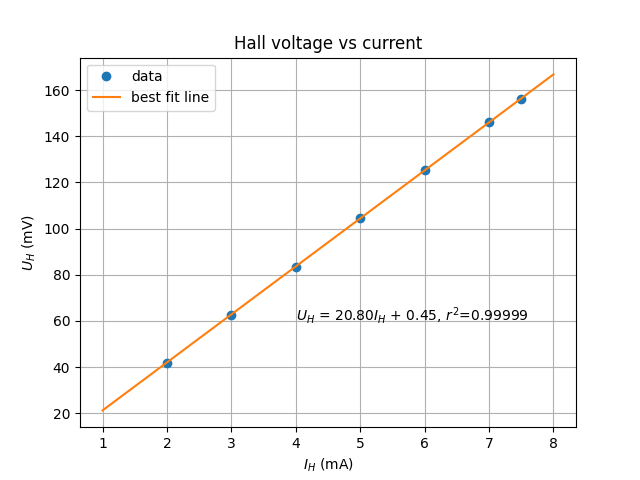
\includegraphics[width=0.6\textwidth]{img/Hall_voltage_vs_current.png}
        \caption{$U_H$-$I_H$关系图}
        \label{U_H-I_H}
    \end{figure}
\end{center}

得到$U_H$与$I_H$的关系为:$U_H = 20.80I_H + 0.45$,其中$R^2$=0.9999,可以认为是线性关系。

计算$a(20.80)$和$b(0.45)$的不确定度:

$$\sigma_a=a\cdot\sqrt{\frac{r^{-2}-1}{n-2}}=20.80\cdot\sqrt{\frac{0.9999^{-2}-1}{7-2}}=0.1315$$

$$\sigma_b=\sigma_a\cdot\sqrt{\frac{\sum x_i^2}{n}}=0.1315\cdot\sqrt{\frac{2^2+3^2+4^2+5^2+6^2+7^2+7.5^2}{7}}=0.7103$$

$$K_H=\frac{U_H}{I_HB_0}=\frac{20.9}{121.1\times10^{-3}}=0.172\times10^{3}m^2/C$$

不确定度计算:$$\sigma_{K_H}=K_H\cdot\sqrt{\left(\frac{\sigma_a}{a}\right)^2+\left(\frac{\sigma_{B_0}}{B_0}\right)^2}=0.172\times10^{3}\cdot\sqrt{\left(\frac{0.1315}{20.80}\right)^2+\left(\frac{0.1}{121.1}\right)^2}=0.001\times10^{3}m^2/C$$

故$$K_H=(0.172\pm0.001)\times10^{3}m^2/C$$

$$R_H=K_H\cdot d=\frac{20.9}{121.1\times10^{-3}}\times3\times10^{-6}=0.516\times10^{-3}m^3/C$$

不确定度计算:$$\sigma_{R_H}=R_H\cdot\sqrt{\left(\frac{\sigma_a}{a}\right)^2+\left(\frac{\sigma_d}{d}\right)^2}=0.516\times10^{-3}\cdot\sqrt{\left(\frac{0.1315}{20.80}\right)^2+\left(\frac{0.1}{3}\right)^2}=0.003\times10^{-3}m^3/C$$

故$$R_H=(0.516\pm0.003)\times10^{-3}m^3/C$$

$$n=\frac{1}{R_H\cdot e}=\frac{1}{0.516\times10^{-3}\times1.6\times10^{-19}}=1.21\times10^{22}m^{-3}$$

不确定度计算:$$\sigma_n=n\cdot\sqrt{\left(\frac{\sigma_{R_H}}{R_H}\right)^2+\left(\frac{\sigma_e}{e}\right)^2}=1.21\times10^{22}\cdot\sqrt{\left(\frac{0.003\times10^{-3}}{0.516\times10^{-3}}\right)^2+\left(\frac{0.1}{1.6\times10^{-19}}\right)^2}=0.02\times10^{22}m^{-3}$$

故$$n=(1.21\pm0.02)\times10^{22}m^{-3}$$

\subsubsection{判断霍尔片的载流子类型}

如图所示,分析霍尔片的载流子类型

\begin{center}
    \begin{figure}[H]
        \centering
        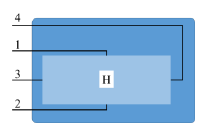
\includegraphics[width=0.4\textwidth]{img/Hall_effect_type.png}
        \caption{霍尔片载流子类型分析图}
        \label{Hall_effect_type}
    \end{figure}
\end{center}

在实验中,磁场方向垂直于直面向内。当$3$接正,$4$接负时,测得$1$点的电势低于$2$点,说明$1$点的电子数目多于$2$点,即这个半导体样品为$N$型半导体。

\subsubsection{标定电磁铁磁隙间磁场}

工作电流$I_H$ = 4.00 mA

实验数据:

\begin{center}
    \begin{tabular}{|c|c|c|c|c|c|c|c|c|c|c|c|}
        \hline
        $I_M$ (mA) & 0 & 100 & 200 & 300 & 400 & 500 & 600 & 700 & 800 & 900 & 1000 \\\hline
        $U_1(B,I)$ (mV) & -13.9 & -30.4 & -46.8 & -63.5 & -80.3 & -96.9 & -113.6 & -130.0 & -146.2 & -162.4 & -178.2 \\\hline
        $U_2(B,-I)$ (mV) & 15.7 & 32.4 & 48.8 & 65.8 & 82.5 & 99.0 & 115.8 & 132.2 & 148.5 & 164.8 & 180.7 \\\hline
        $U_3(-B,-I)$ (mV) & 16.0 & -1.5 & -18.1 & -34.8 & -51.6 & -68.2 & -84.8 & -101.2 & -117.5 & -133.7 & -149.8 \\\hline
        $U_4(-B,I)$ (mV) & -14.1 & 3.4 & 20.0 & 36.7 & 53.4 & 70.0 & 86.7 & 103.0 & 119.0 & 135.5 & 151.7 \\\hline
        $U_H$ (mV) & 0.1 & 16.2 & 33.4 & 50.2 & 66.9 & 83.5 & 100.2 & 116.6 & 132.8 & 149.1 & 165.1 \\\hline
    \end{tabular}
    \begin{minipage}{0.8\textwidth}
        \centering
        \fontsize{9pt}{\baselineskip}\selectfont
        表2\quad 霍尔电压测量数据表
    \end{minipage}
    \label{Hall_voltage_data}
\end{center}

利用公式$K_H=\dfrac{U_H}{I_HB_0}$,得到$B=\dfrac{U_H}{I_HK_H}$,计算对应的磁感应强度$B$得以下数据

\begin{center}
    \begin{tabular}{|c|c|c|c|c|c|c|c|c|c|c|c|}
        \hline
        $I_M$ (mA) & 0 & 100 & 200 & 300 & 400 & 500 & 600 & 700 & 800 & 900 & 1000 \\\hline
        $U_H$ (mV) & 0.1 & 16.2 & 33.4 & 50.2 & 66.9 & 83.5 & 100.2 & 116.6 & 132.8 & 149.1 & 165.1 \\\hline
        $B$ (mT) & 0.1 & 23.5 & 48.5 & 73.0 & 97.2 & 121.3 & 145.6 & 169.5 & 193.0 & 216.7 & 240.0 \\\hline
    \end{tabular}
    \begin{minipage}{0.8\textwidth}
        \centering
        \fontsize{9pt}{\baselineskip}\selectfont
        表3\quad 磁场强度测量数据表
    \end{minipage}
    \label{Magnetic_field_data}
\end{center}

如图所示,用最小二乘法拟合:

\begin{center}
    \begin{figure}[H]
        \centering
        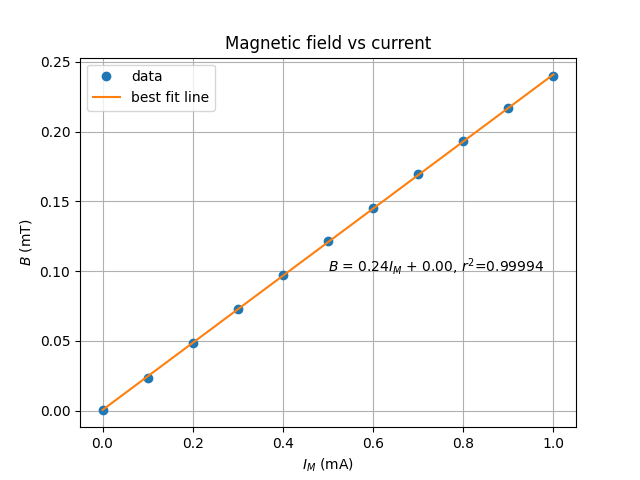
\includegraphics[width=0.6\textwidth]{img/Magnetic_field_vs_current.png}
        \caption{$B$-$I_M$关系图}
        \label{B-I_M}
    \end{figure}
\end{center}

得到$B$与$I_M$的关系为:$B = 0.24I_M + 0.00$,其中$R^2$=0.9999,可以认为是线性关系。

计算$a(0.24)$和$b(0.00)$的不确定度:

$$\sigma_a=a\cdot\sqrt{\frac{r^{-2}-1}{n-2}}=0.24\cdot\sqrt{\frac{0.9999^{-2}-1}{12-2}}=0.0004$$

$$\sigma_b=\sigma_a\cdot\sqrt{\frac{\sum x_i^2}{n}}=0.0004\cdot\sqrt{\frac{0^2+100^2+200^2+300^2+400^2+500^2+600^2+700^2+800^2+900^2+1000^2}{12}}=0.0555$$

\subsubsection{测定磁极间隙磁场分布}

条件:$I_H$ = 4.00 mA,$I_M$ = 500 mA

实验数据:

\begin{center}
    \begin{tabular}{|c|c|c|c|c|c|c|c|c|}
        \hline
        $x$ (mm) & 0.0 & 4.0 & 6.0 & 8.0 & 10.0 & 12.0 & 17.0 & 22.0 \\\hline
        $U_1(B,I)$ (mV) & -49.2 & -71.2 & -85.5 & -94.1 & -97.0 & -97.7 & -97.7 & -97.4 \\\hline
        $U_2(B,-I)$ (mV) & 51.2 & 73.3 & 87.6 & 96.2 & 99.1 & 99.8 & 99.8 & 99.5 \\\hline
        $U_3(-B,-I)$ (mV) & -20.1 & -42.2 & -56.5 & -65.1 & -68.0 & -68.7 & -68.6 & -68.4 \\\hline
        $U_4(-B,I)$ (mV) & 22.0 & 44.0 & 58.4 & 67.0 & 69.9 & 70.5 & 70.2 & 69.9 \\\hline
        $U_H$ (mV) & 35.6 & 57.6 & 72.0 & 80.6 & 83.5 & 84.1 & 84.1 & 83.8 \\\hline
        \hline
        $x$ (mm) & 28.0 & 33.0 & 38.0 & 40.0 & 42.0 & 44.0 & 46.0 & 50.0\\\hline
        $U_1(B,I)$ (mV) & -97.0 & -96.7 & -96.4 & -96.1 & -95.0 & -91.4 & -82.2 & -56.4 \\\hline
        $U_2(B,-I)$ (mV) & 99.2 & 98.9 & 98.6 & 98.2 & 97.2 & 93.5 & 84.3 & 68.4 \\\hline
        $U_3(-B,-I)$ (mV) & -68.0 & -67.7 & -67.4 & -67.1 & -66.0 & -62.4 & -53.1 & -27.3 \\\hline
        $U_4(-B,I)$ (mV) & 69.9 & 69.6 & 69.2 & 68.9 & 67.9 & 64.2 & 55.0 & 29.2 \\\hline
        $U_H$ (mV) & 83.5 & 83.2 & 82.9 & 82.6 & 81.5 & 77.9 & 68.7 & 45.3 \\\hline
    \end{tabular}
    \begin{minipage}{0.8\textwidth}
        \centering
        \fontsize{9pt}{\baselineskip}\selectfont
        表4\quad 磁场分布测量数据表
    \end{minipage}
    \label{Hall_voltage_distribution_data}
\end{center}

对数据进行处理,计算出磁场:

\begin{center}
    \begin{tabular}{|c|c|c|c|c|c|c|c|c|c|c|c|}
        \hline
        $x$ (mm) & 0.0 & 4.0 & 6.0 & 8.0 & 10.0 & 12.0 & 17.0 & 22.0 \\\hline
        $U_H$ (mV) & 35.6 & 57.6 & 72.0 & 80.6 & 83.5 & 84.1 & 84.1 & 83.8 \\\hline
        $B$ (mT) & 51.7 & 83.7 & 104.7 & 117.2 & 121.4 & 122.2 & 122.2 & 121.8 \\\hline
        \hline
        $x$ (mm) & 28.0 & 33.0 & 38.0 & 40.0 & 42.0 & 44.0 & 46.0 & 50.0\\\hline
        $U_H$ (mV) & 83.5 & 83.2 & 82.9 & 82.6 & 81.5 & 77.9 & 68.7 & 45.3 \\\hline
        $B$ (mT) & 121.4 & 120.9 & 120.5 & 120.1 & 118.5 & 113.2 & 99.8 & 65.8 \\\hline
    \end{tabular}
    \begin{minipage}{0.8\textwidth}
        \centering
        \fontsize{9pt}{\baselineskip}\selectfont
        表5\quad 磁场分布测量数据表
    \end{minipage}
    \label{Magnetic_field_distribution_data}
\end{center}

做图如下:

\begin{center}
    \begin{figure}[H]
        \centering
        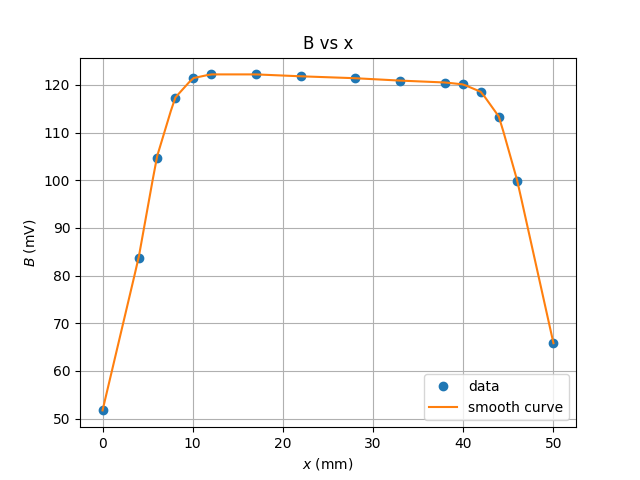
\includegraphics[width=0.6\textwidth]{img/Magnetic_field_distribution.png}
        \caption{磁场分布图}
        \label{Magnetic_field_distribution}
    \end{figure}
\end{center}

\subsubsection{测量霍尔片载流子迁移率$\mu$}

长方形霍尔片的尺寸:$l$ = 300$\mu$m,$b$ = 100$\mu$m,$d$ = 3$\mu$m,$I_H$ = 4.00 mA,$I_M$ = 0 mA

实验数据:

\begin{center}
    \begin{tabular}{|c|c|c|c|c|c|}
        \hline
        工作电流$I_H$ (mA) & 0.50 & 1.00 & 1.50 & 2.00 & 2.50 \\\hline
        电流方向压降$U$ (V) & 0.3796 & 0.7672 & 1.1507 & 1.5286 & 1.9132 \\\hline
    \end{tabular}
    \begin{minipage}{0.8\textwidth}
        \centering
        \fontsize{9pt}{\baselineskip}\selectfont
        表6\quad 电流方向压降测量数据表
    \end{minipage}
\end{center}

如图所示,用最小二乘法拟合:

\begin{center}
    \begin{figure}[H]
        \centering
        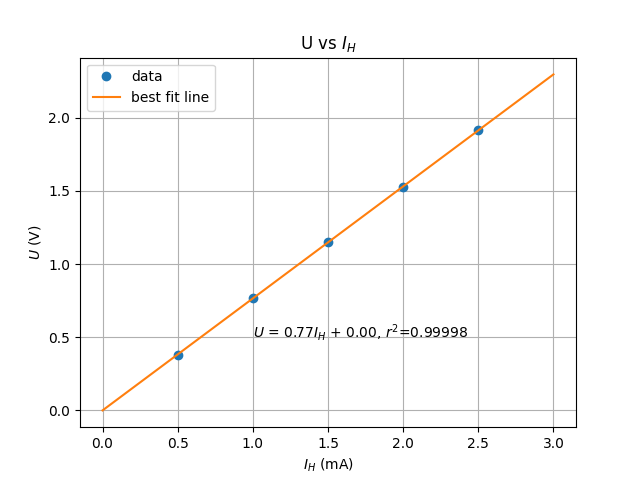
\includegraphics[width=0.6\textwidth]{img/Current_vs_voltage.png}
        \caption{$U$-$I_H$关系图}
        \label{U-I_H}
    \end{figure}
\end{center}

得到$U$与$I_H$的关系为:$U = 0.77I_H + 0.00$,其中$R^2$=0.9999,可以认为是线性关系。

计算$a(0.77)$和$b(0.00)$的不确定度:

$$\sigma_a=a\cdot\sqrt{\frac{r^{-2}-1}{n-2}}=0.77\cdot\sqrt{\frac{0.9999^{-2}-1}{5-2}}=0.0062$$

$$\sigma_b=\sigma_a\cdot\sqrt{\frac{\sum x_i^2}{n}}=0.0009\cdot\sqrt{\frac{0.5^2+1^2+1.5^2+2^2+2.5^2}{5}}=0.0009$$

由定义可知:$$\mu=\frac{v}{E}=K_H\frac{I_Hl}{bU}=K_H\frac{I_H}{U}\frac{l}{b}$$

带入数值计算得:$$\mu=0.172\times10^{3}\times\frac{1}{0.77}\times\frac{300\times10^{-6}}{100\times10^{-6}}=670.1cm^2/V\cdot s$$

计算不确定度:

\begin{equation}
    \begin{aligned}
        \sigma{\mu}
        & = \mu\cdot\sqrt{\left(\frac{\sigma_{K_H}}{K_H}\right)^2+\left(\frac{\sigma_{I_H}}{I_H}\right)^2+\left(\frac{\sigma_{U}}{U}\right)^2+\left(\frac{\sigma_{l}}{l}\right)^2+\left(\frac{\sigma_{b}}{b}\right)^2}\\
        & = 670.1\cdot\sqrt{\left(\frac{0.001\times10^{3}}{0.172\times10^{3}}\right)^2+\left(\frac{0.1}{1}\right)^2+\left(\frac{0.0009}{0.77}\right)^2+\left(\frac{0.1}{300}\right)^2+\left(\frac{0.1}{100}\right)^2}\\
        & = 4.3cm^2/V\cdot s\\
    \end{aligned}
\end{equation}

故$$\mu=(670.1\pm4.3)cm^2/V\cdot s$$

\subsection{磁电阻特性测量}

实验条件:$I_{CD}$ = 1.50 mA,$AB$端短路。调节样品架水平、竖直位置,使磁阻片位于磁隙中央

实验数据:

\begin{center}
    \begin{tabular}{|c|c|c|c|c|c|c|c|c|}
        \hline
        $I_M$ (mA) & 0 & 50 & 100 & 150 & 200 & 250 & 300 & 350 \\\hline
        $U_{CD}$ (V) & 0.5434 & 0.5506 & 0.5704 & 0.6017 & 0.6406 & 0.6859 & 0.7341 & 0.7803 \\\hline
        $B$ (mT) & 0.0 & 12.0 & 24.0 & 36.0 & 48.0 & 60.0 & 72.0 & 84.0 \\\hline
        $R_B$ ($\Omega$) & 362.3 & 367.1 & 380.3 & 401.1 & 427.1 & 458.6 & 489.4 & 520.2 \\\hline
        $\Delta R/R(0)$ & 0.0000 & 0.0132 & 0.0497 & 0.1071 & 0.1788 & 0.2658 & 0.3508 & 0.4358 \\\hline
        \hline
        $I_M$ (mA) & 400 & 500 & 600 & 700 & 800 & 900 & 1000 & \~{}\\\hline
        $U_{CD}$ (V) & 0.8160 & 0.8648 & 0.9011 & 0.9345 & 0.9665 & 0.9958 & 1.0262 & \~{} \\\hline
        $B$ (mT) & 96.0 & 120.0 & 144.0 & 168.0 & 192.0 & 216.0 & 240.0 & \~{} \\\hline
        $R_B$ ($\Omega$) & 544.0 & 576.5 & 600.7 & 623.0 & 645.7 & 666.5 & 684.1 & \~{} \\\hline
        $\Delta R/R(0)$ & 0.5015 & 0.5912 & 0.6580 & 0.7196 & 0.7822 & 0.8296 & 0.8882 & \~{} \\\hline
    \end{tabular}
    \begin{minipage}{0.8\textwidth}
        \centering
        \fontsize{9pt}{\baselineskip}\selectfont
        表7\quad 磁电阻特性测量数据表
    \end{minipage}
\end{center}

做图如下:

\begin{center}
    \begin{figure}[H]
        \centering
        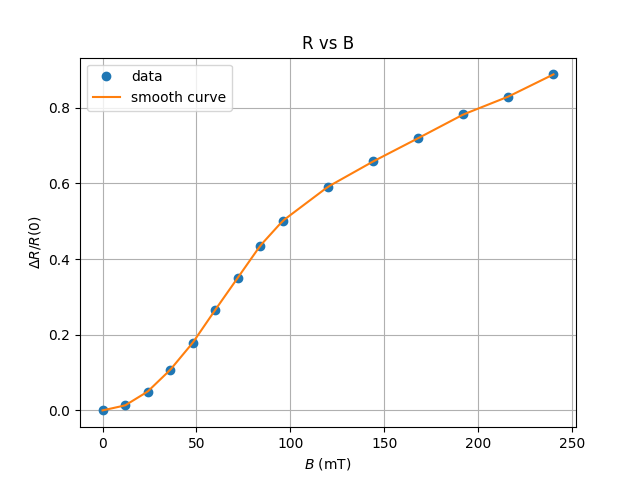
\includegraphics[width=0.6\textwidth]{img/Magnetoresistance.png}
        \caption{磁电阻特性曲线}
        \label{Magnetoresistance}
    \end{figure}
\end{center}

可以看出,在磁感应强度小于100mT时,$\Delta R/R(0)$成二次函数关系,当磁感应强度大于100mT时,$\Delta R/R(0)$成一次函数关系。

即磁电阻的阻值在低磁场下成二次函数关系,而在高磁场下成一次函数关系。

\section{实验小结}

\begin{enumerate}
    \item 了解了霍尔效应及其副效应的产生原理
    \item 掌握了霍尔系数的测量方法
    \item 学习并实际操作了消除霍尔副效应的实验方法
    \item 研究了半导体材料的电阻值随磁场的变化规律
\end{enumerate}

\newpage
\section{教师签字的原始实验数据}
    \begin{center}
        \begin{figure}[H] %H为当前位置,!htb为忽略美学标准,htbp为浮动图形
            \centering %图片居中
            \includegraphics[width=0.8\textwidth]{img/OriginalData1.jpg} %插入图片,[]中设置图片大小,{}中是图片文件名
            \caption{原始数据1} %最终文档中希望显示的图片标题
            \label{原始数据-1} %用于文内引用的标签
        \end{figure}
        \begin{figure}[H] %H为当前位置,!htb为忽略美学标准,htbp为浮动图形
            \centering %图片居中
            \includegraphics[width=0.8\textwidth]{img/OriginalData2.jpg} %插入图片,[]中设置图片大小,{}中是图片文件名
            \caption{原始数据2} %最终文档中希望显示的图片标题
            \label{原始数据-2} %用于文内引用的标签
        \end{figure}
    \end{center}
\end{document}
